\documentclass[12pt,a4paper]{article}
\usepackage[UTF8]{ctex}
\usepackage{amsmath,amssymb}
\usepackage{xcolor}
\usepackage{hyperref}
\usepackage{geometry}
\usepackage{graphicx}
\geometry{margin=2.5cm}

\title{Diffusion Operator / 扩散算子}
\author{QuoNic}
\date{}

\begin{document}
\maketitle

\begin{center}
\textbf{Algorithms / 算法} | 难度：中级 | 预计时间：10 分钟
\end{center}

\tableofcontents
\newpage

\section{为什么需要？}

扩散算子是 Grover 搜索的核心组件。

\subsection{经典局限}
\begin{itemize}
  \item 经典搜索需要 $O(N)$ 次查询
  \item 对于大规模问题，经典方法效率低
\end{itemize}

\subsection{量子优势}
\begin{itemize}
  \item 扩散算子可以放大目标态的振幅
  \item 是 Grover 搜索的核心
  \item 提供二次加速
\end{itemize}

\subsection{实际应用}
\begin{itemize}
  \item Grover 搜索
  \item 振幅放大
  \item 量子优化
\end{itemize}

\section{快速上手}

\begin{verbatim}
from quonic.algorithms import diffusion
result = diffusion(n_qubits=2)
print(f'Operator: {result.operator}')
\end{verbatim}

\textbf{预期输出}：
\begin{verbatim}
Operator: [[-0.5, 0.5, 0.5, 0.5], ...]
\end{verbatim}

\section{原理详解}

\subsection{电路图}

\begin{center}
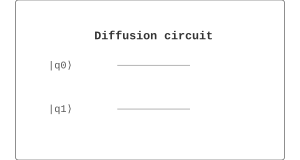
\includegraphics[width=0.6\textwidth]{../../images/diffusion_circuit.svg}
\end{center}

\subsection{数学推导}

扩散算子关于平均振幅反射：
\begin{equation}
D = 2|s\rangle\langle s| - I
\end{equation}

其中 $|s\rangle$ 是均匀叠加态。

\textbf{作用}：
\begin{equation}
D|\psi\rangle = 2\langle s|\psi\rangle|s\rangle - |\psi\rangle
\end{equation}

\subsection{几何解释}

扩散算子在 Bloch 球上关于平均振幅反射，放大目标态的振幅。

\section{代码详解}

\begin{verbatim}
from quonic.algorithms import diffusion

# diffusion(n_qubits)
# n_qubits: number of qubits
result = diffusion(n_qubits=2)
print(f'Operator: {result.operator}')
\end{verbatim}

\section{进阶用法}

\subsection{场景 1：不同量子比特数}

\begin{verbatim}
from quonic.algorithms import diffusion
for n in [2, 3, 4]:
    result = diffusion(n_qubits=n)
    print(f'n={n}: {result.operator.shape}')
\end{verbatim}

\section{适用场景}

\subsection{Grover 搜索}

扩散算子是 Grover 搜索的核心组件。

\subsection{振幅放大}

扩散算子用于振幅放大算法。

\section{常见问题}

\subsection{扩散算子的作用是什么？}

关于平均振幅反射，放大目标态的振幅。

\subsection{扩散算子和 Oracle 有什么区别？}

Oracle 标记目标态，扩散算子放大目标态的振幅。

\section{学习路径}

\subsection{前置知识}
\begin{itemize}
  \item Grover 搜索
  \item 振幅放大
  \item 量子测量
\end{itemize}

\subsection{继续学习}
\begin{itemize}
  \item 量子计数
  \item 量子优化
  \item 量子算法
\end{itemize}

\section{完整示例代码}

\subsection{示例 1：基本扩散算子}

\begin{verbatim}
from quonic.algorithms import diffusion
result = diffusion(n_qubits=2)
print(f'Operator: {result.operator}')
\end{verbatim}

\section{下载}

\begin{itemize}
  \item [diffusion.py](https://github.com/ChrisLee0721/QuoNic/blob/main/examples/diffusion/diffusion.py)
\end{itemize}

\end{document}
